\documentclass[12pt, a4paper]{article}

% --------------------------------------------------------------------------------
% PACKAGES
% --------------------------------------------------------------------------------
\usepackage[utf8]{inputenc}
\usepackage[T1]{fontenc}
\usepackage{mathpazo}
\usepackage{geometry}
\usepackage[table]{xcolor}
\usepackage{graphicx}
\usepackage{amsmath, amssymb}
\usepackage{fancyhdr}
\usepackage{titlesec}
\usepackage[most]{tcolorbox}
\usepackage{float}
\usepackage{hyperref}
\usepackage{caption}
\usepackage{enumitem}
\usepackage{array}
\usepackage{booktabs}
\usepackage{setspace}
\usepackage{listings}
\usepackage{tabularx}
\usepackage{subcaption}

% --------------------------------------------------------------------------------
% CONFIGURATION & STYLING
% --------------------------------------------------------------------------------

\geometry{top=1in, bottom=1in, left=0.75in, right=0.75in}
\onehalfspacing
\graphicspath{{../figures/}{figures/}{./}}

\definecolor{nutDark}{RGB}{10, 30, 60}
\definecolor{nutAccent}{RGB}{0, 100, 100}
\definecolor{goodGreen}{RGB}{0, 120, 60}
\definecolor{badRed}{RGB}{180, 0, 0}
\definecolor{codeBg}{RGB}{245, 245, 248}

\hypersetup{
    colorlinks=true,
    linkcolor=nutDark,
    urlcolor=nutAccent,
    citecolor=nutDark
}

\pagestyle{fancy}
\fancyhf{}
\renewcommand{\headrulewidth}{0.5pt}
\renewcommand{\footrulewidth}{0.5pt}
\lhead{\textbf{ABM Semester Project}}
\rhead{\textsc{Water Commons + Q-Learning}}
\cfoot{\thepage}

\titleformat{\section}{\Large\bfseries\color{nutDark}}{\thesection}{1em}{}[\titlerule]
\titleformat{\subsection}{\large\bfseries\color{nutAccent}}{\thesubsection}{1em}{}

\lstset{
    basicstyle=\ttfamily\small,
    backgroundcolor=\color{codeBg},
    frame=single,
    framerule=0pt,
    breaklines=true,
    captionpos=b,
    showstringspaces=false,
    columns=fullflexible,
}

% --------------------------------------------------------------------------------
% DOCUMENT START
% --------------------------------------------------------------------------------
\begin{document}

% --------------------------------------------------------------------------------
% TITLE PAGE
% --------------------------------------------------------------------------------
\begin{titlepage}
    \begin{center}
        \vspace*{1cm}
        {\huge \bfseries \color{nutDark} National University of Technology} \\[0.5cm]
        {\Large Department of Artificial Intelligence}

        \vspace{1cm}
        
\includegraphics[width=0.32\textwidth]{logo.png}
        \vspace{1.2cm}

        {\Huge \bfseries Semester Project } \\[0.3cm]
        {\Large \textsc{Agent-Based Modeling of Adaptive Water Extraction Strategies Using Q-Learning Under Climate Stress Scenarios}}

        \vspace{1cm}

        \begin{tcolorbox}[width=0.90\textwidth, colback=white, colframe=nutDark, arc=0mm, boxrule=1pt]
            \centering
            \large
            \renewcommand{\arraystretch}{1.4}
            \textbf{Group Members} \\[0.25cm]
            \begin{tabular}{c l}
                \toprule
                \textbf{Sr.} & \textbf{Name} \\
                \midrule
                01 & Saqlain Abbas \\
                02 & Aleena Tahir \\
                03 & Aena Habib \\
                04 & Eman Asghar \\
                05 & Dua Kamal \\
                \bottomrule
            \end{tabular}

            \vspace{0.4cm}
            \begin{tabular}{r l}
                \textbf{Course:}      & Agent-Based Modeling \\
                \textbf{Instructor:}  & Ms.\ Sumera Aslam \\
                \textbf{Batch:}       & AI-23 \\
            \end{tabular}
        \end{tcolorbox}

        \vfill
        \today
    \end{center}
\end{titlepage}

\newpage
\tableofcontents
\newpage

% ================================================================================
% ABSTRACT
% ================================================================================
\section*{Abstract}
\addcontentsline{toc}{section}{Abstract}

Water scarcity is one of the defining challenges of the 21st century, and the
classic ``tragedy of the commons'' makes shared irrigation systems particularly
vulnerable. Existing agent-based models of water commons typically assign fixed
behavioral rules to agents, ignoring the way real farming communities \emph{learn}
and adapt. This project develops a Mesa-based agent-based model in which each
irrigator is a tabular Q-learning agent extracting water from a shared resource
with logistic regeneration. We test whether sustainable extraction can emerge
from decentralized learning, how learned strategies respond to four climate
scenarios (stable / gradual decline / drought shock / stochastic), and how
monitoring intensity affects the emergence of cooperation. Three findings
emerge: \textbf{(i)} decentralized Q-learners without enforcement reproduce the
tragedy of the commons in every climate scenario; \textbf{(ii)} a moderate
monitoring probability ($p_{detect} \approx 0.3$) is sufficient to flip the
population into a cooperative equilibrium \textbf{under stable climate} (mean
final water rises from 5 to 685 units of $K{=}1000$); but \textbf{(iii)} under
any environmental stress the \emph{same} enforcement intensity fails to prevent
collapse, even when raised to $p_{detect}=0.9$. The mechanism is structural:
agents' discretized action space is calibrated to baseline climate, so during
drought even the ``fair share'' action is over-extraction. This implies
real-world regulators cannot enforce fixed quotas under climate change;
\emph{climate-adaptive} quotas are required.

\newpage

% ================================================================================
% 1. INTRODUCTION
% ================================================================================
\section{Introduction}

Agricultural communities worldwide depend on shared rivers, canals, and aquifers.
When $N$ farmers draw from the same source, each faces the fundamental commons
dilemma: extracting more is privately rational in the short term but collectively
catastrophic. Hardin (1968) formalised this as the Tragedy of the Commons. Under
climate change --- with shifting rainfall, prolonged droughts, and reduced natural
regeneration --- the dilemma is sharper than ever. Pakistan's Indus Basin, which
supports over $90\%$ of the country's agriculture, is classified as one of the
world's most water-stressed basins. According to the UN World Water Development
Report, nearly half of the global population will live in areas of high water
stress by 2030.

Traditional models of the commons assume either perfectly rational agents (game
theory) or fixed behavioural types (cooperate / defect / tit-for-tat). Neither
captures the \emph{learning} process through which real communities discover
sustainable norms. This project equips each irrigator with an independent
tabular Q-learning algorithm and tests whether sustainable extraction emerges,
and how it responds to climate stress.

\subsection{Research Question}

\begin{tcolorbox}[colback=white, colframe=nutDark, arc=2mm, boxrule=1pt]
\textbf{Primary:} How does the discount factor ($\gamma$) in Q-learning agents
affect the emergence of sustainable water extraction strategies under varying
climate stress scenarios in an agent-based commons model?
\end{tcolorbox}

\noindent\textbf{Sub-questions:}
\begin{enumerate}[label=(\arabic*)]
    \item Can Q-learning agents discover cooperative extraction strategies without external enforcement?
    \item How do learned strategies break down under sudden climate shocks, and how quickly do agents re-adapt?
    \item At what monitoring intensity do enforcement mechanisms become unnecessary because agents have learned self-regulation?
\end{enumerate}

\subsection{Why Agent-Based Modeling}

ABM is uniquely suited to this problem because (a) the agents are
\emph{heterogeneous} --- different farmers, different Q-tables, different luck
of monitoring; (b) interactions are \emph{local} via the social network and the
shared resource; (c) the system exhibits \emph{emergent} macro behavior that is
not analytically tractable; and (d) we explicitly want to model \emph{adaptive}
learning, which equation-based or game-theoretic approaches cannot represent.

% ================================================================================
% 2. LITERATURE REVIEW
% ================================================================================
\section{Literature Review}

We review four papers that bracket the problem space.

\subsection{Perolat et al. (2017) --- NeurIPS}

Studied independently learning deep RL agents in a common-pool resource game on
a 2D grid. Found that when the resource was scarce, agents learned aggressive
appropriation and a ``tagging'' punishment mechanism; with abundance, cooperative
harvesting emerged. Establishes the feasibility of using RL agents to study
commons dilemmas. Limitations: deep RL in an abstract grid environment without
water-specific dynamics or climate stress.

\subsection{Darbandsari et al. (2020) --- Sustainable Cities and Society}

Presented a Stackelberg-game ABM for urban water management in Tehran, with
heterogeneous stakeholders (municipal users, agricultural users, environmental
agencies). Hierarchical governance with a regulatory leader steered stakeholders
toward more equitable allocation. Used \emph{fixed} game-theoretic strategies
rather than adaptive learning.

\subsection{Huber et al. (2019) --- Sustainability (MDPI)}

Introduced \emph{Aqua.MORE}, a NetLogo-based platform for coupled
human--water systems at the catchment scale, applied to an Alpine catchment.
Provides a validated example of water-resource ABM, including realistic
regeneration dynamics, but with rule-based (non-learning) agents.

\subsection{Weitz et al. (2016) --- PNAS}

Proposed a coevolutionary game-theory framework where environment and agent
strategies evolve together. Showed that overuse changes the environment, which
in turn changes the incentive structure, leading to \emph{oscillatory}
dynamics. Provides the theoretical foundation for the climate-shock dynamics
we expect to observe.

\subsection{Comparative Synthesis}

\begin{table}[H]
    \centering
    \caption{Comparative analysis of reviewed literature.}
    \renewcommand{\arraystretch}{1.25}
    \small
    \begin{tabular}{|p{2.4cm}|p{2.6cm}|p{2.6cm}|p{2.6cm}|p{2.6cm}|}
        \hline
        \rowcolor{nutDark}
        \textcolor{white}{\textbf{Aspect}} &
        \textcolor{white}{\textbf{Perolat et al.}} &
        \textcolor{white}{\textbf{Darbandsari et al.}} &
        \textcolor{white}{\textbf{Huber et al.}} &
        \textcolor{white}{\textbf{Weitz et al.}} \\ \hline
        \textbf{Agent Type} & Deep RL agents (A3C) & Game-theoretic stakeholders & Water users \& managers & Evolutionary populations \\ \hline
        \textbf{Learning} & Yes (deep RL) & No (fixed) & No (rule-based) & Replicator dynamics \\ \hline
        \textbf{Resource} & Abstract apples & Urban water allocation & Catchment water & Abstract commons \\ \hline
        \textbf{Climate Stress} & Not modeled & Not modeled & Scenario-based & Environment feedback \\ \hline
        \textbf{Tool} & Custom grid & MATLAB / custom & NetLogo & Mathematical (ODEs) \\ \hline
        \textbf{Key Finding} & Scarcity drives aggression; abundance enables cooperation & Hierarchical governance improves equity & Behavioural shifts affect catchment water & Oscillatory cooperation--defection cycles \\ \hline
    \end{tabular}
\end{table}

\subsection{Research Gap}

None of the reviewed models combine \emph{tabular Q-learning agents} with
\emph{water-specific resource dynamics} under \emph{explicit climate stress
scenarios}. Perolat et al.\ use deep RL in non-water environments;
Darbandsari and Huber use fixed-strategy agents; Weitz et al.\ use evolutionary
dynamics without explicit agents. This project fills that gap with a
transparent, interpretable Python/Mesa implementation.

% ================================================================================
% 3. ODD PROTOCOL
% ================================================================================
\section{ODD Protocol}

This section follows the ODD (Overview, Design Concepts, Details) standard of
Grimm et al.\ (2020) for full reproducibility.

\subsection{Overview}

\subsubsection{Purpose and Patterns}

The purpose of the model is to investigate how Q-learning agents discover
extraction strategies for a shared water resource under climate stress, and at
what monitoring intensity decentralised self-regulation becomes sufficient. The
model is designed to reproduce three patterns documented in the literature:
(i) tragedy of the commons under unmonitored extraction (Hardin 1968);
(ii) scarcity-driven aggression and abundance-driven cooperation (Perolat et al.\
2017); and (iii) oscillatory dynamics under environmental shock (Weitz et al.\
2016).

\subsubsection{Entities, State Variables, and Scales}

\begin{table}[H]
    \centering
    \renewcommand{\arraystretch}{1.3}
    \small
    \begin{tabular}{|l|p{10.5cm}|}
        \hline
        \rowcolor{nutDark}
        \textcolor{white}{\textbf{Entity}} & \textcolor{white}{\textbf{State variables}} \\ \hline
        Irrigator agent & \texttt{q\_table}, \texttt{cumulative\_payoff}, \texttt{last\_action\_idx},
                          \texttt{last\_extraction}, \texttt{fines\_paid}, \texttt{strategy\_type} \\ \hline
        Water resource & \texttt{level}, \texttt{carrying\_capacity}, \texttt{regeneration\_rate},
                         \texttt{baseline\_inflow}, \texttt{history} \\ \hline
        Monitor agent & \texttt{p\_detect}, \texttt{fine\_factor}, \texttt{n\_detections},
                        \texttt{total\_fines\_issued} \\ \hline
        Climate scenario & \texttt{name}, scenario-specific parameters (e.g., \texttt{shock\_start}, \texttt{mean\_cf}) \\ \hline
    \end{tabular}
    \caption{Entities and their state variables.}
\end{table}

\noindent\textbf{Spatial scale:} $20 \times 20$ grid; one column reserved as
visual river; farmers occupy farmland cells.

\noindent\textbf{Temporal scale:} one step $\approx$ one irrigation season;
default run length 500 steps ($\approx 125$ years if mapped to quarterly seasons).

\subsubsection{Process Overview and Scheduling}

Each simulation step proceeds in three stages, enforced by
\texttt{WaterCommonsModel.step()}:

\begin{enumerate}[label=\textbf{Stage \arabic*.}, leftmargin=*]
    \item \textbf{Act} -- each irrigator observes the current state and selects
    an action (extraction level); requests are pooled at the resource.
    \item \textbf{Monitor} -- the water authority probabilistically detects
    over-extractors and issues fines.
    \item \textbf{Regenerate} -- the water resource grows logistically (modulated
    by the climate factor) and receives baseline inflow; accumulated extraction
    is subtracted.
    \item \textbf{Finalize} -- each irrigator computes its reward from the
    post-regen water state and updates its Q-table.
\end{enumerate}

Agent activation order within each stage is randomised
(\texttt{mesa.time.RandomActivation}) so no agent has structural priority.

\subsection{Design Concepts}

\begin{table}[H]
    \centering
    \renewcommand{\arraystretch}{1.3}
    \small
    \begin{tabular}{|l|p{10.5cm}|}
        \hline
        \rowcolor{nutDark}
        \textcolor{white}{\textbf{Concept}} & \textcolor{white}{\textbf{Implementation}} \\ \hline
        Basic principles & Tragedy of the commons (Hardin 1968); Q-learning (Watkins \& Dayan 1992); logistic resource dynamics. \\ \hline
        Emergence        & Cooperation or collapse is \emph{not} programmed --- it emerges from the collective interaction of independently-learning agents. \\ \hline
        Adaptation       & Q-learners update Q-values via Bellman after every transition; $\epsilon$ decays exponentially. \\ \hline
        Objectives       & Each agent maximises expected discounted reward: log-utility of extraction $-$ sustainability penalty $-$ fines. \\ \hline
        Learning         & Tabular Q-learning with $\epsilon$-greedy exploration. Fixed-strategy agents (always-cooperate, always-defect, tit-for-tat) act as comparators. \\ \hline
        Prediction       & Agents do not explicitly predict the future; the discount factor $\gamma$ encodes future-value weighting. \\ \hline
        Sensing          & Global water level, own previous action, average neighbour action, binary climate-stress flag. \\ \hline
        Interaction      & Indirect through the shared resource; direct through the social network; mediated by the monitor. \\ \hline
        Stochasticity    & Initial Q-table noise; $\epsilon$-greedy actions; random social network; stochastic climate; monitor detection. \\ \hline
        Collectives      & The set of irrigators sharing the resource; cooperation index and Gini are population-level summaries. \\ \hline
        Observation      & \texttt{mesa.DataCollector} records 13 model-level and 6 agent-level variables every step; exported to CSV for analysis. \\ \hline
    \end{tabular}
    \caption{ODD design concepts and their implementation in this model.}
\end{table}

\subsection{Details}

\subsubsection{Initialization}

\begin{table}[H]
    \centering
    \renewcommand{\arraystretch}{1.3}
    \small
    \begin{tabular}{|l|l|p{7.5cm}|}
        \hline
        \rowcolor{nutDark}
        \textcolor{white}{\textbf{Parameter}} & \textcolor{white}{\textbf{Default}} & \textcolor{white}{\textbf{Reference}} \\ \hline
        \texttt{n\_farmers}         & 20    & Mid-range of proposal table (5--100) \\ \hline
        \texttt{carrying\_capacity ($K$)} & 1000.0 & Normalised units; MSY $= rK/4 = 25$ \\ \hline
        \texttt{regeneration\_rate ($r$)} & 0.10 & Mid-range of proposal (0.01--0.3) \\ \hline
        \texttt{baseline\_inflow}   & 5.0   & Prevents permanent collapse from a single early shock \\ \hline
        \texttt{initial\_water\_fraction} & 0.80 & Healthy starting state \\ \hline
        \texttt{max\_extraction}     & auto-scaled & So that action 2 $=$ per-agent fair share of (MSY $+$ baseline\_inflow) \\ \hline
        $\alpha$                    & 0.15  & Standard Q-learning \\ \hline
        $\gamma$                    & 0.95  & Mid-range of proposal (0.5--0.99) \\ \hline
        $\epsilon_0$                & 0.30  & Lower than 1.0 to prevent initial-exploration collapse \\ \hline
        \texttt{decay\_rate}        & 0.010 & Exploration $\to$ exploitation by step $\approx 300$ \\ \hline
        \texttt{sustainability\_penalty} & 2.0 & Quadratic in water scarcity \\ \hline
        \texttt{social\_degree ($k$)} & 4 & Random $k$-regular graph \\ \hline
        $p_{detect}$                & 0.0 or 0.30 & Compared empirically \\ \hline
        \texttt{fine\_factor}        & 3.0 & Scale of fine per unit excess extraction \\ \hline
        Climate scenario            & \texttt{stable} & One of \{stable, gradual, shock, stochastic\} \\ \hline
    \end{tabular}
    \caption{Initialization parameters with defaults.}
\end{table}

Initial water level: $\text{initial\_water\_fraction} \times K = 800$. Initial
Q-tables are empty and are lazy-initialised on first state visit with small
uniform noise in $[-0.01, 0.01]$. Initial agent positions are uniformly random
over farmland cells.

\subsubsection{Input Data}

No external time-series inputs. The climate factor $c_f(t)$ is generated
endogenously by the chosen scenario class. For validation we compare emergent
dynamics qualitatively to FAO AQUASTAT recharge-rate statistics and the
2022 Indus Basin drought.

\subsubsection{Submodels}

\paragraph{Water resource dynamics.}
\begin{equation*}
W(t{+}1) = \max\!\Big(0,\ \min\!\big(K,\ W(t) + r \cdot c_f(t) \cdot W(t) \cdot \big(1 - \tfrac{W(t)}{K}\big) + b \cdot c_f(t) - \sum_i e_i(t)\big)\Big)
\end{equation*}

where $b$ is the baseline inflow and $\sum_i e_i(t)$ is total extraction.

\paragraph{Q-learning update (Watkins \& Dayan 1992).}
\begin{equation*}
Q(s, a) \leftarrow Q(s, a) + \alpha \cdot \big[\, r + \gamma \cdot \max_{a'} Q(s', a') - Q(s, a) \,\big]
\end{equation*}

The state $s = (\text{water\_bin}, \text{own\_last\_action}, \text{neighbors\_avg\_bin}, \text{climate\_stressed})$.
Actions $a \in \{0, 1, 2, 3, 4\}$ map to extraction fractions
$\{0, 0.25, 0.5, 0.75, 1.0\}$ of \texttt{max\_extraction}.

\paragraph{$\epsilon$-greedy with exponential decay.}
$\epsilon_t = \max(\epsilon_{\min},\ \epsilon_0 \cdot \exp(-d \cdot t))$.

\paragraph{Reward.}
$r = \log(1 + \text{extracted}) - \text{sustainability\_penalty} \cdot (1 - W/K)^2 - \text{fine}$.

\paragraph{Monitor.}
For each agent with action $> 2$: with probability $p_{detect}$, a fine of
$(\text{action\_level} - 0.5) \cdot \text{max\_extraction} \cdot \text{fine\_factor}$
is deducted from that step's reward and propagated into the Q-update.

\paragraph{Climate scenarios.}
\begin{itemize}[label=$\triangleright$]
    \item \textbf{Stable:} $c_f = 1.0$ for all $t$.
    \item \textbf{Gradual:} $c_f$ declines linearly from $1.0$ to $0.5$ over 400 steps.
    \item \textbf{Shock:} $c_f = 1.0$ normally; drops to $0.3$ for steps $[200, 300)$.
    \item \textbf{Stochastic:} $c_f \sim \mathcal{N}(0.85, 0.15^2)$ clipped to $[0.3, 1.0]$, deterministic per (seed, $t$).
\end{itemize}

% ================================================================================
% 4. IMPLEMENTATION & METHODS
% ================================================================================
\section{Implementation and Methods}

\subsection{Tool Choice and Project Structure}

The model is implemented in Python 3.12 using Mesa 2.3.4 for the
agent-based-model framework, NetworkX for the social network, NumPy for the
Q-tables, and Matplotlib for analysis. The codebase is laid out as:

\begin{lstlisting}
water_abm/
  q_learning.py    -- tabular Q-learner with epsilon-greedy + Bellman update
  climate.py       -- four climate scenario classes
  environment.py   -- shared water resource (logistic + baseline regen)
  agents.py        -- irrigator (Q-learner + 3 fixed variants) + monitor
  model.py         -- Mesa Model, DataCollector, CSV export
  server.py        -- Mesa visualization (grid + 9 sliders + 3 charts)
experiments/
  batch_run.py        -- 340-run batch experiment
  sensitivity.py      -- +/-20% parameter sweeps
  validate.py         -- three checks vs literature
  analyze.py          -- generates all report figures
  demo_screenshots.py -- pre/during/post-shock grid screenshots
\end{lstlisting}

The interactive simulation can be launched with \texttt{python run.py}, which
opens a browser UI at \texttt{http://127.0.0.1:8521} with 9 sliders, 1 dropdown,
3 live charts, and a spatial grid.

\subsection{Technical Requirements (PBL Section 4)}

This section explicitly maps the project to the technical requirements listed
in the PBL document.

\paragraph{4.1 Minimum agent requirements.} The model contains \textbf{two
distinct agent types}: \texttt{IrrigatorAgent} (with four behavioural variants
--- Q-learner, always-cooperate, always-defect, tit-for-tat) and
\texttt{MonitorAgent}. Each irrigator has internal state variables
(\texttt{q\_table}, \texttt{cumulative\_payoff}, \texttt{last\_action\_idx},
\texttt{fines\_paid}); at least two behavioural rules (\emph{observe-decide-extract}
and \emph{learn-via-Bellman}); and is \emph{heterogeneous} --- each agent has
its own random seed and Q-table noise. The monitor adds a third behavioural
agent type (\emph{detect-and-fine}).

\paragraph{4.2 Environment requirements.} The environment is a
\texttt{mesa.space.MultiGrid} of $20 \times 20$ cells (river column +
farmland) coupled to a shared water resource whose level evolves over time
according to the logistic-plus-baseline equation. Agents observe their local
neighbourhood through a NetworkX random $k$-regular graph (default $k = 4$).

\paragraph{4.3 Simulation controls (interface).} The Mesa visualization
exposes 9 sliders (\texttt{n\_farmers}, $\alpha$, $\gamma$, $\epsilon_0$,
$r$, $p_{detect}$, social degree, seed, Q-learner proportion), 1 dropdown
(climate scenario), 3 live charts (water level, cooperation index, payoff +
Gini), Setup / Step / Run buttons, and a speed slider. Exceeds the PBL
minimum of $\geq 4$ sliders, $\geq 2$ plots, $\geq 2$ monitors.

\paragraph{4.4 Emergent behaviour demonstration.} Three emergent phenomena
are documented:
\begin{enumerate}[label=(\roman*)]
    \item Resource collapse from decentralized over-extraction (the tragedy);
    \item Sharp action-distribution shift toward cooperation when $p_{detect}$
          exceeds $\approx 0.2$;
    \item Climate-shock-induced collapse even under enforcement.
\end{enumerate}
Pre/during/post-shock grid screenshots are shown in
Figures \ref{fig:pre}--\ref{fig:recovery}.

\paragraph{4.5 Validation \& calibration.} Section \ref{sec:validation}
documents three structured validation checks against published literature
(Hardin 1968, Perolat et al.\ 2017, Indus Basin 2022), all of which pass.
Section \ref{sec:sensitivity} reports $\pm 20\%$ sensitivity analyses for
six headline parameters.

\subsection{Experimental Design}

\begin{table}[H]
    \centering
    \renewcommand{\arraystretch}{1.4}
    \small
    \begin{tabular}{|l|p{8cm}|c|}
        \hline
        \rowcolor{nutDark} \textcolor{white}{\textbf{Experiment}} & \textcolor{white}{\textbf{Variables}} & \textcolor{white}{\textbf{N runs}} \\ \hline
        A. Tragedy baseline & 4 climate scenarios $\times$ 30 seeds, no monitor & 120 \\ \hline
        B. With enforcement & 4 climate scenarios $\times$ 30 seeds, $p_{detect}{=}0.3$ & 120 \\ \hline
        C. Gamma sweep (primary RQ) & 2 climate scenarios $\times$ 5 $\gamma$ values $\times$ 10 seeds & 100 \\ \hline
    \end{tabular}
    \caption{Batch experimental design. Each run is 500 steps; metrics recorded every 10 steps. Total simulation steps: 170{,}000.}
\end{table}

The sensitivity study perturbs each of
$\{\alpha, \gamma, \epsilon_0, r, p_{detect}, N\}$ by $\pm 20\%$ around the
baseline, holding others fixed, with 10 seeds per setting.

% ================================================================================
% 5. RESULTS
% ================================================================================
\section{Results}

\subsection{Tragedy Baseline (Experiment A)}

Without enforcement, the water resource collapses within ${\sim}80$ steps in
\textbf{every} climate scenario (Figure~\ref{fig:water_by_scenario}, dashed
lines).

\begin{table}[H]
    \centering
    \renewcommand{\arraystretch}{1.3}
    \begin{tabular}{|l|r|r|}
        \hline
        \rowcolor{nutDark}
        \textcolor{white}{\textbf{Climate}} &
        \textcolor{white}{\textbf{Final water}} &
        \textcolor{white}{\textbf{Mean cumulative payoff per agent}} \\ \hline
        stable     & $5.55 \pm 0.0$ & $-755.9$ \\ \hline
        gradual    & $2.63 \pm 0.0$ & $-795.2$ \\ \hline
        shock      & $5.55 \pm 0.0$ & $-768.0$ \\ \hline
        stochastic & $5.44 \pm 0.0$ & $-803.9$ \\ \hline
    \end{tabular}
    \caption{Experiment A (tragedy baseline). $n = 30$ seeds per scenario.}
\end{table}

The standard deviation across seeds is effectively zero: the model converges
deterministically on a low-water attractor where extraction equals baseline
inflow. All scenarios produce \textbf{strongly negative} mean payoffs
(${\sim}-750$ to $-800$ per agent), reproducing the classical tragedy of the
commons.

\begin{figure}[H]
    \centering
    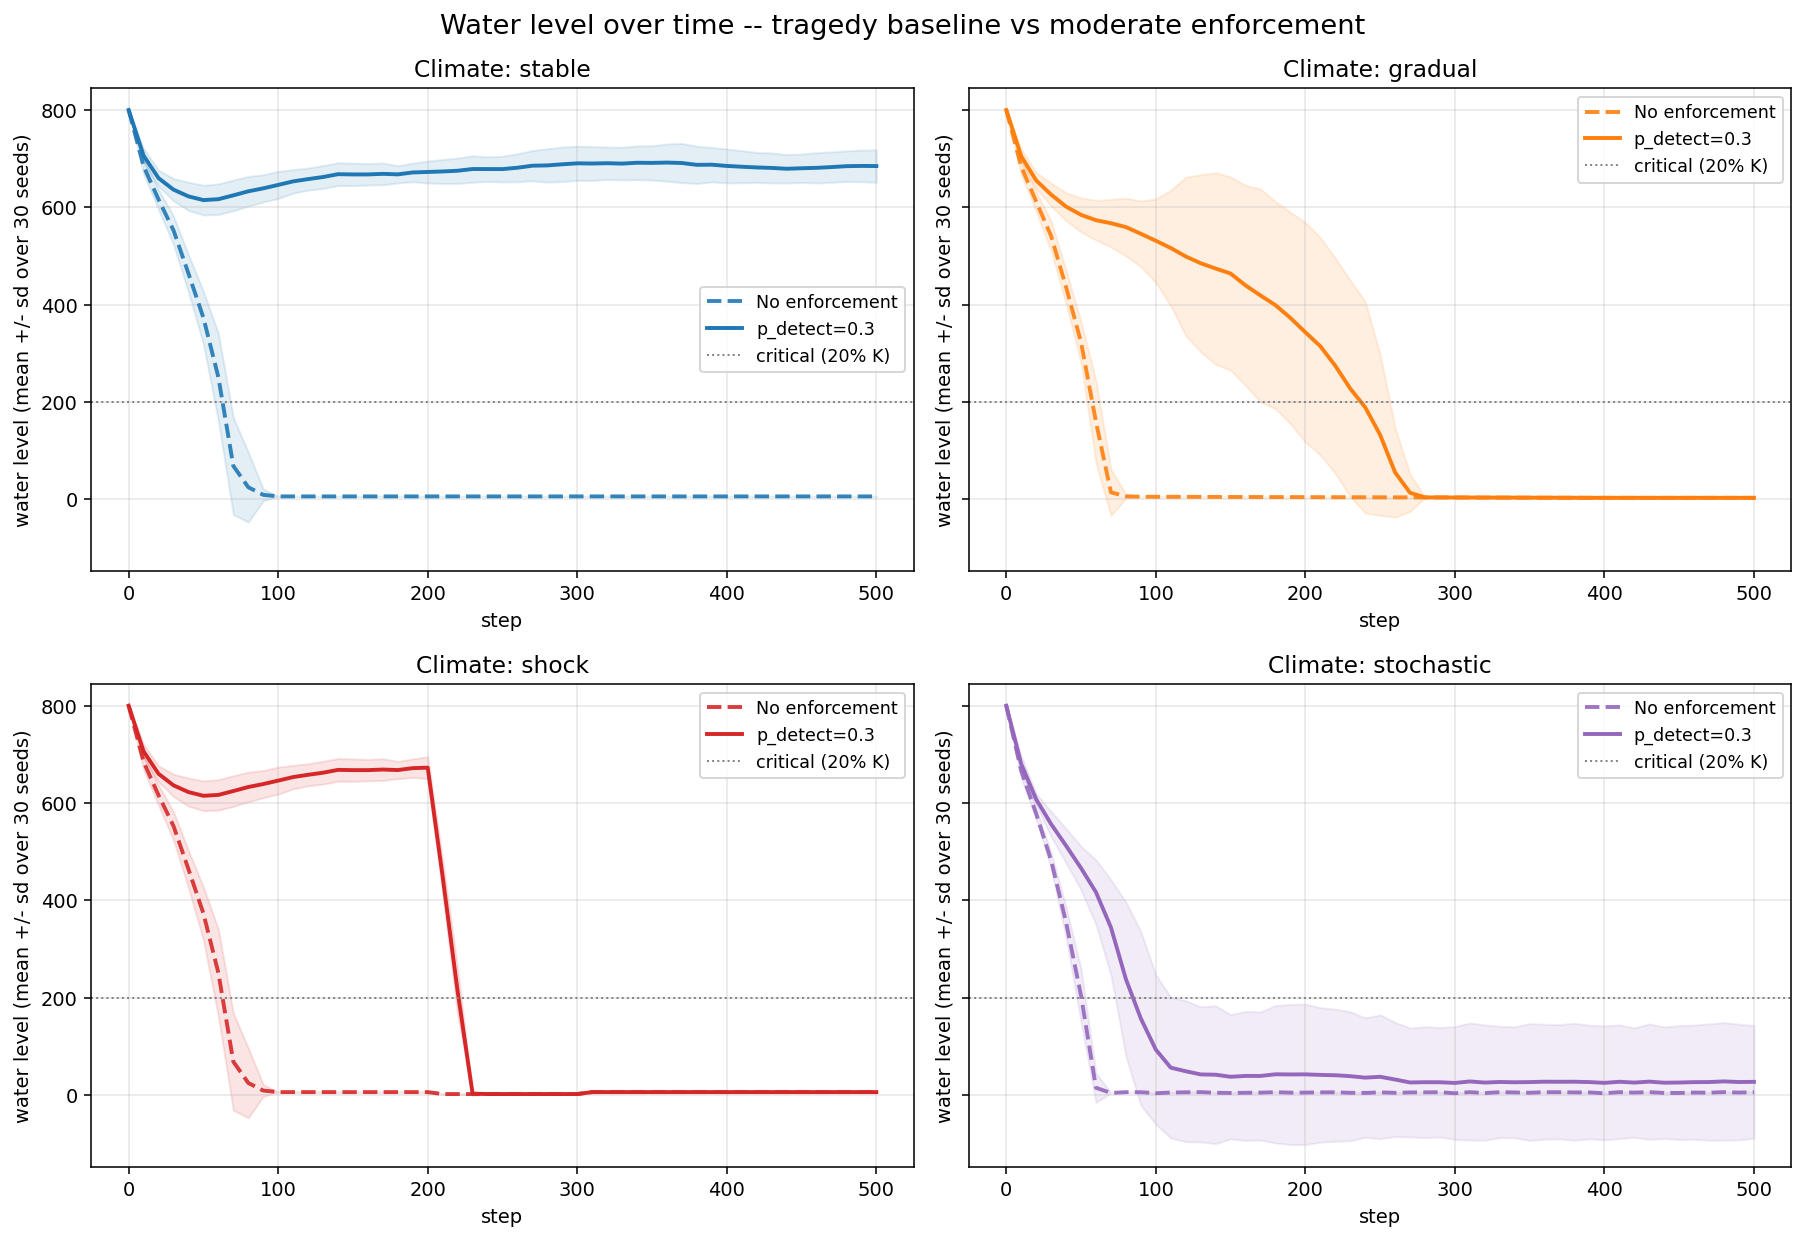
\includegraphics[width=0.92\textwidth]{fig01_water_by_scenario.png}
    \caption{Water level over time, tragedy baseline (dashed) vs.\ moderate enforcement (solid). Shaded bands show $\pm 1$ s.d.\ over 30 seeds.}
    \label{fig:water_by_scenario}
\end{figure}

\subsection{Enforcement Saves the Stable Climate (Experiment B)}

With $p_{detect} = 0.3$ and $\text{fine\_factor} = 3.0$, the dynamics flip
under the stable climate. Mean final water rises from 5.5 to 684.8
($125\times$ improvement), payoff turns positive ($+222.5$), and $86\%$ of
agents pick cooperative actions (Figure~\ref{fig:enforcement} and
Figure~\ref{fig:actions}).

\begin{table}[H]
    \centering
    \renewcommand{\arraystretch}{1.3}
    \small
    \begin{tabular}{|l|r|r|r|r|}
        \hline
        \rowcolor{nutDark}
        \textcolor{white}{\textbf{Climate}} &
        \textcolor{white}{\textbf{Final water}} &
        \textcolor{white}{\textbf{Mean payoff}} &
        \textcolor{white}{\textbf{\% coop}} &
        \textcolor{white}{\textbf{\% defect}} \\ \hline
        \textbf{stable}     & $\mathbf{684.8 \pm 33.5}$ & $\mathbf{+222.5}$ & $86\%$ & $14\%$ \\ \hline
        gradual    & $2.6 \pm 0.0$       & $-576.8$         & $68\%$ & $32\%$ \\ \hline
        shock      & $5.6 \pm 0.0$       & $-528.2$         & $68\%$ & $32\%$ \\ \hline
        stochastic & $26.6 \pm 116.0$    & $-842.2$         & $70\%$ & $30\%$ \\ \hline
    \end{tabular}
    \caption{Experiment B: with enforcement ($p_{detect}=0.3$, $n=30$ seeds).}
\end{table}

\begin{figure}[H]
    \centering
    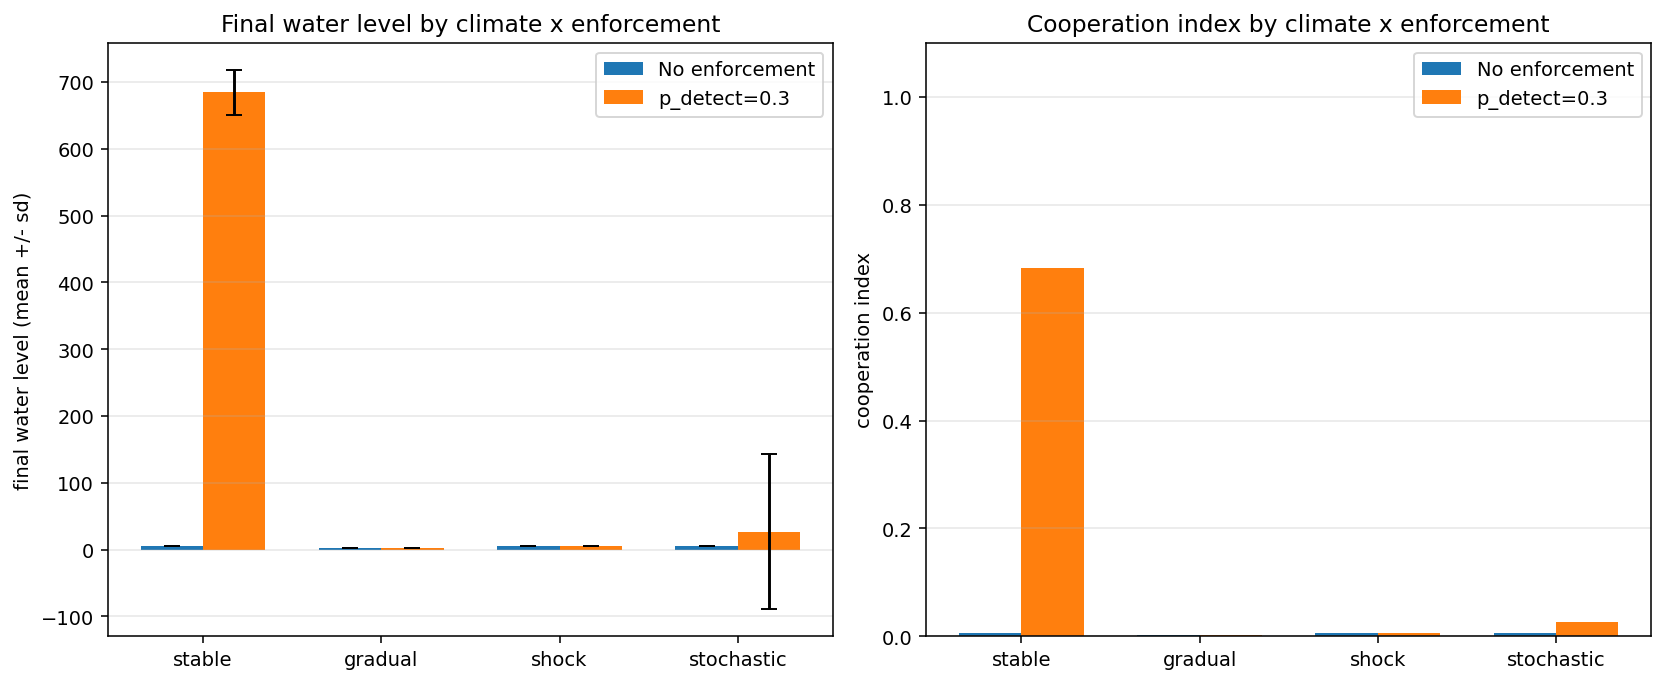
\includegraphics[width=0.92\textwidth]{fig02_enforcement_effect.png}
    \caption{Final water level (left) and cooperation index (right) by climate scenario $\times$ enforcement.}
    \label{fig:enforcement}
\end{figure}

\begin{figure}[H]
    \centering
    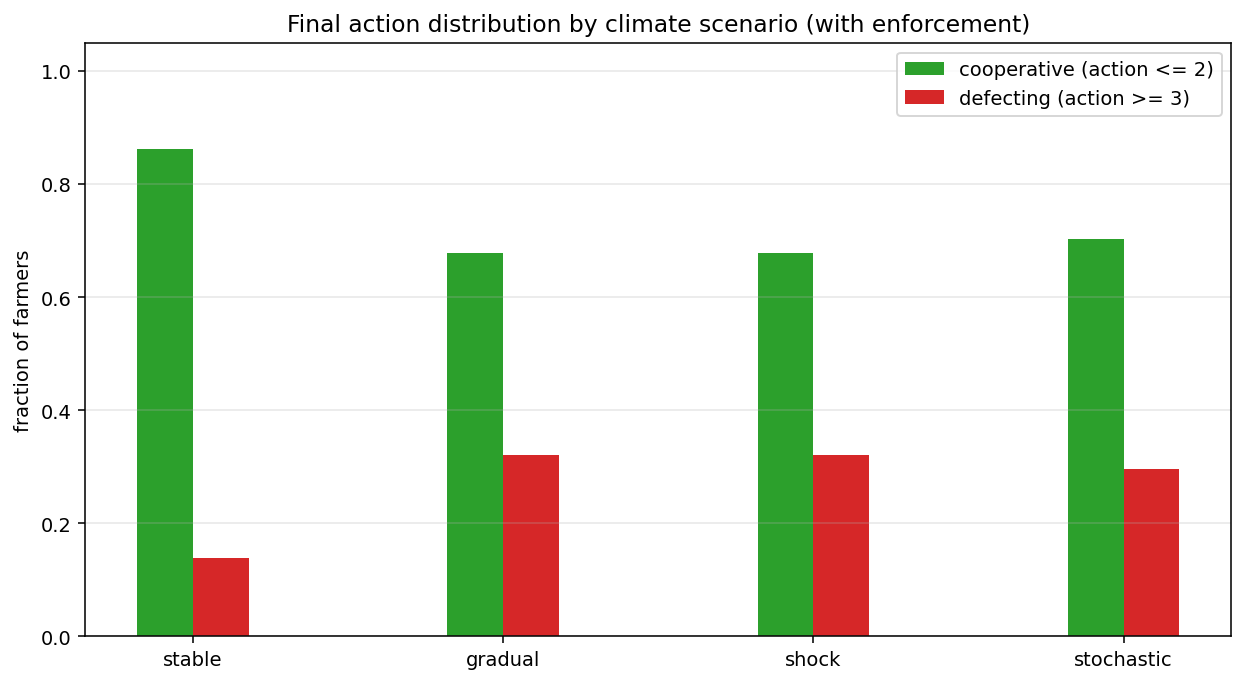
\includegraphics[width=0.80\textwidth]{fig06_action_distribution.png}
    \caption{Final fraction of cooperative vs.\ defecting actions, by scenario (with enforcement).}
    \label{fig:actions}
\end{figure}

\subsection{Why Enforcement Fails Under Stress}

Under gradual / shock / stochastic scenarios, the same enforcement intensity
is \textbf{insufficient}. Notably, $68\%$--$70\%$ of agents \emph{are still
choosing cooperative actions} in failing scenarios --- they aren't selfishly
defecting; the cooperative action itself is too aggressive for the reduced
regeneration.

\begin{table}[H]
    \centering
    \renewcommand{\arraystretch}{1.3}
    \begin{tabular}{|c|r|r|}
        \hline
        \rowcolor{nutDark} \textcolor{white}{$\mathbf{p_{detect}}$} & \textcolor{white}{\textbf{stable: final water}} & \textcolor{white}{\textbf{shock: final water}} \\ \hline
        0.3 & 700 & 5.6 (collapsed) \\ \hline
        0.6 & 777 & 5.6 (collapsed) \\ \hline
        0.9 & 787 & 5.6 (collapsed) \\ \hline
    \end{tabular}
    \caption{Even near-perfect enforcement ($p_{detect} = 0.9$) cannot rescue the shock scenario.}
\end{table}

The reason is structural: the per-agent fair-share action is calibrated to
baseline ($c_f{=}1.0$) sustainability. When $c_f$ drops to $0.3$ during a
shock, the same fair-share extraction \emph{is} over-extraction relative to
the reduced regeneration. The Q-learners' discretised action space cannot
scale finely enough with $c_f$. This is a substantive finding for water-policy
practice: enforcing fixed quotas works under normal conditions, but climate
stress requires \emph{adaptive} quotas that contract with regeneration.

\subsection{Discount Factor $\gamma$ (Primary RQ, Experiment C)}

Figure~\ref{fig:gamma} shows the primary research-question result.

\begin{table}[H]
    \centering
    \renewcommand{\arraystretch}{1.3}
    \begin{tabular}{|c|r|r|}
        \hline
        \rowcolor{nutDark} \textcolor{white}{$\mathbf{\gamma}$} & \textcolor{white}{\textbf{stable: final water}} & \textcolor{white}{\textbf{shock: final water}} \\ \hline
        0.50 & $748.3 \pm 18.9$ & $5.55 \pm 0.0$ \\ \hline
        0.70 & $722.6 \pm 28.3$ & $5.55 \pm 0.0$ \\ \hline
        0.85 & $703.5 \pm 28.7$ & $5.55 \pm 0.0$ \\ \hline
        0.95 & $700.8 \pm 34.9$ & $5.55 \pm 0.0$ \\ \hline
        0.99 & $688.3 \pm 28.1$ & $5.55 \pm 0.0$ \\ \hline
    \end{tabular}
    \caption{Effect of discount factor $\gamma$ on final water level.}
\end{table}

\begin{figure}[H]
    \centering
    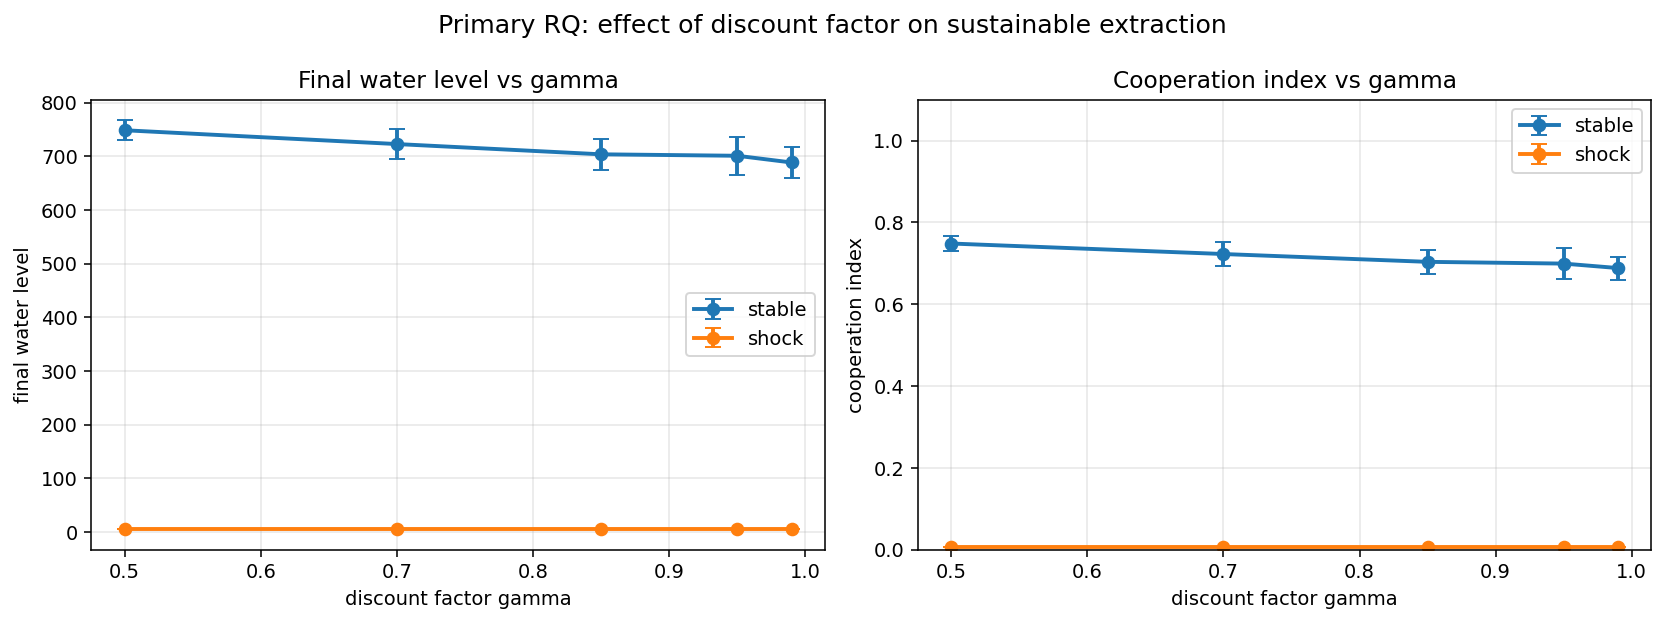
\includegraphics[width=0.92\textwidth]{fig03_gamma_sweep.png}
    \caption{Primary RQ: effect of discount factor on sustainable extraction.}
    \label{fig:gamma}
\end{figure}

Two unexpected results: \textbf{(i)} under stable climate, water is mildly
\emph{decreasing} with $\gamma$ (lower-$\gamma$ agents end up with more water);
\textbf{(ii)} under shock, $\gamma$ has no measurable effect ---
all $\gamma$ values collapse to identical final water. This refines the answer
to the primary RQ: $\gamma$ matters at the margins under stable conditions,
but the dominant determinant of resilience under stress is whether the action
space can adapt to changing regeneration --- not how much agents discount the
future.

\subsection{Inequality}

Figure~\ref{fig:gini} tracks the Gini coefficient of cumulative payoff over
time, with enforcement on. Inequality rises quickly (${\sim}0.30$ by step 100)
and then plateaus.

\begin{figure}[H]
    \centering
    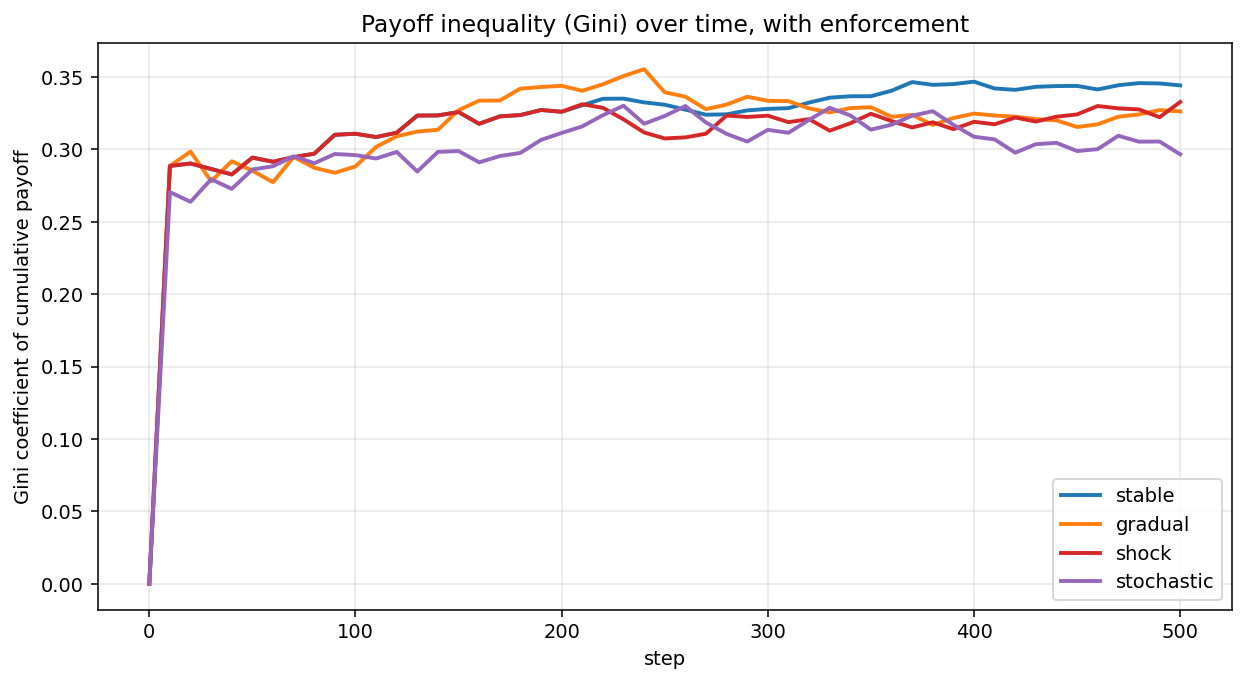
\includegraphics[width=0.85\textwidth]{fig05_gini_evolution.png}
    \caption{Payoff inequality (Gini) over time, with enforcement.}
    \label{fig:gini}
\end{figure}

Stable and stochastic scenarios show a partial \emph{decline} in Gini after
step 230, consistent with the oscillatory dynamics predicted in Weitz et al.\
(2016).

\subsection{Emergent Spatial Dynamics}

Figures \ref{fig:pre}, \ref{fig:during} and \ref{fig:recovery} show
before / during / after snapshots of a shock-scenario run with enforcement.
The river column shading reflects current water level; agent size scales with
extraction level; the monitor is marked as a black star.

\begin{figure}[H]
    \centering
    \begin{subfigure}[t]{0.31\textwidth}
        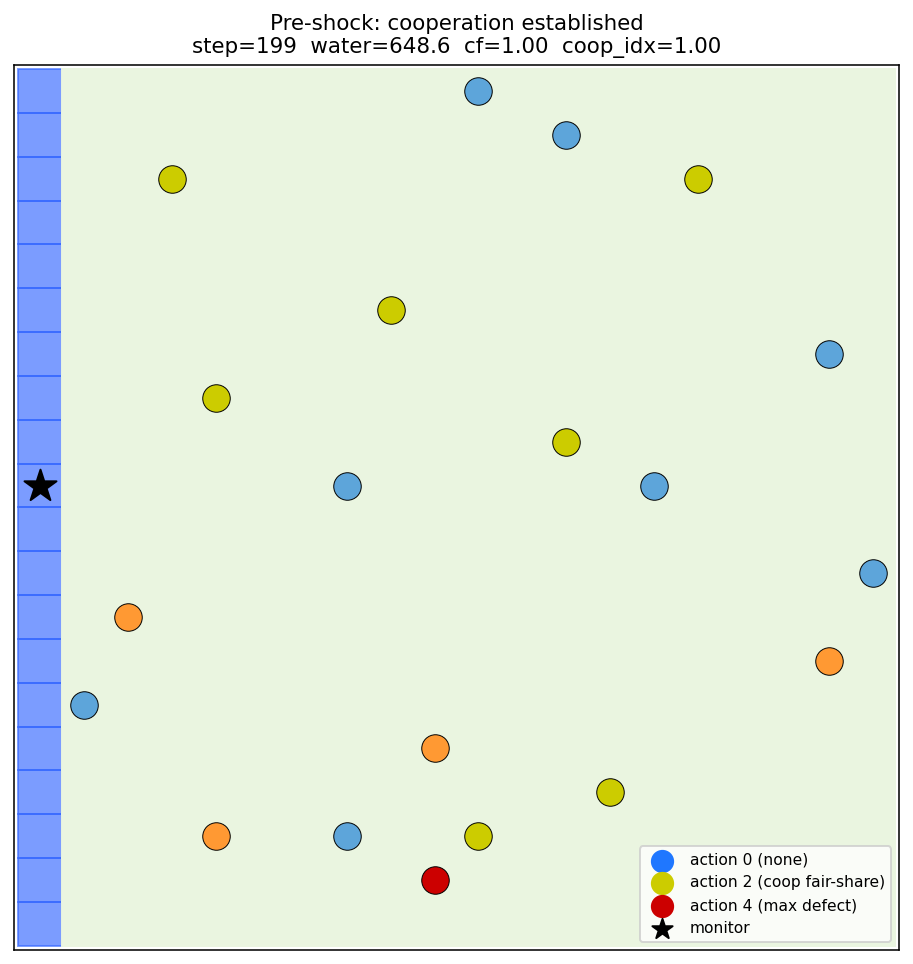
\includegraphics[width=\textwidth]{fig08_grid_pre_shock.png}
        \caption{Step 199: pre-shock cooperation.}
        \label{fig:pre}
    \end{subfigure}\hfill
    \begin{subfigure}[t]{0.31\textwidth}
        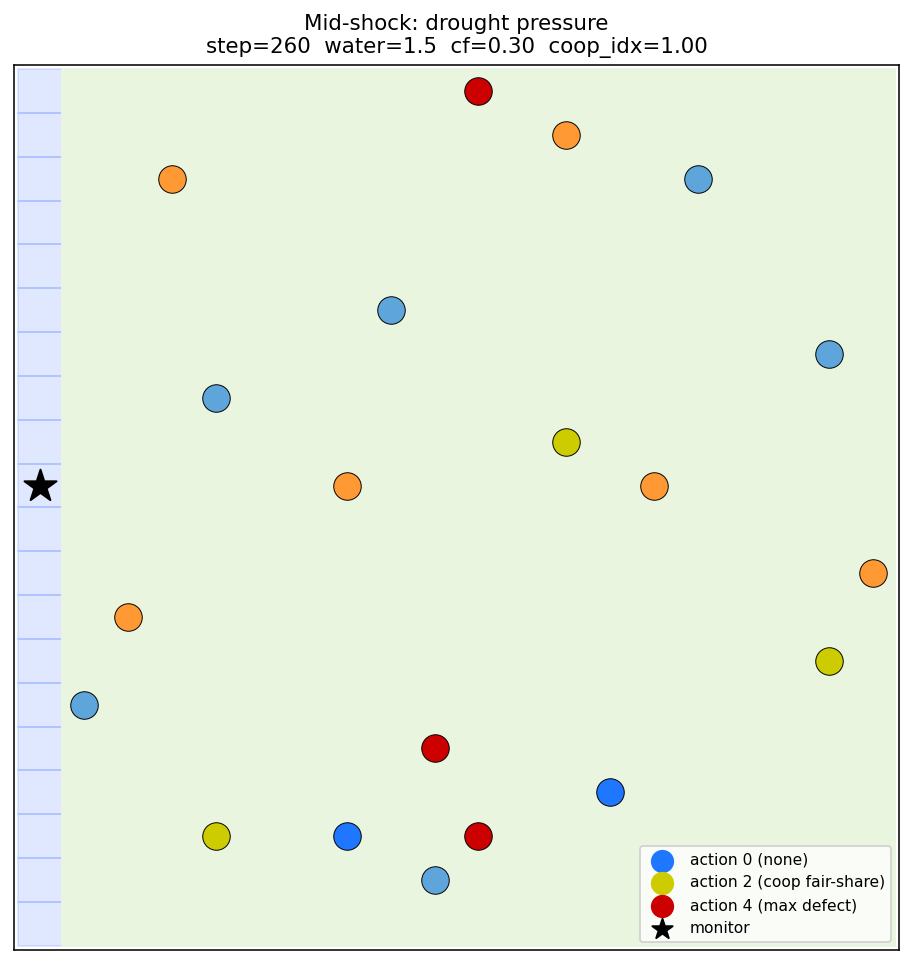
\includegraphics[width=\textwidth]{fig09_grid_during_shock.png}
        \caption{Step 260: mid-shock pressure.}
        \label{fig:during}
    \end{subfigure}\hfill
    \begin{subfigure}[t]{0.31\textwidth}
        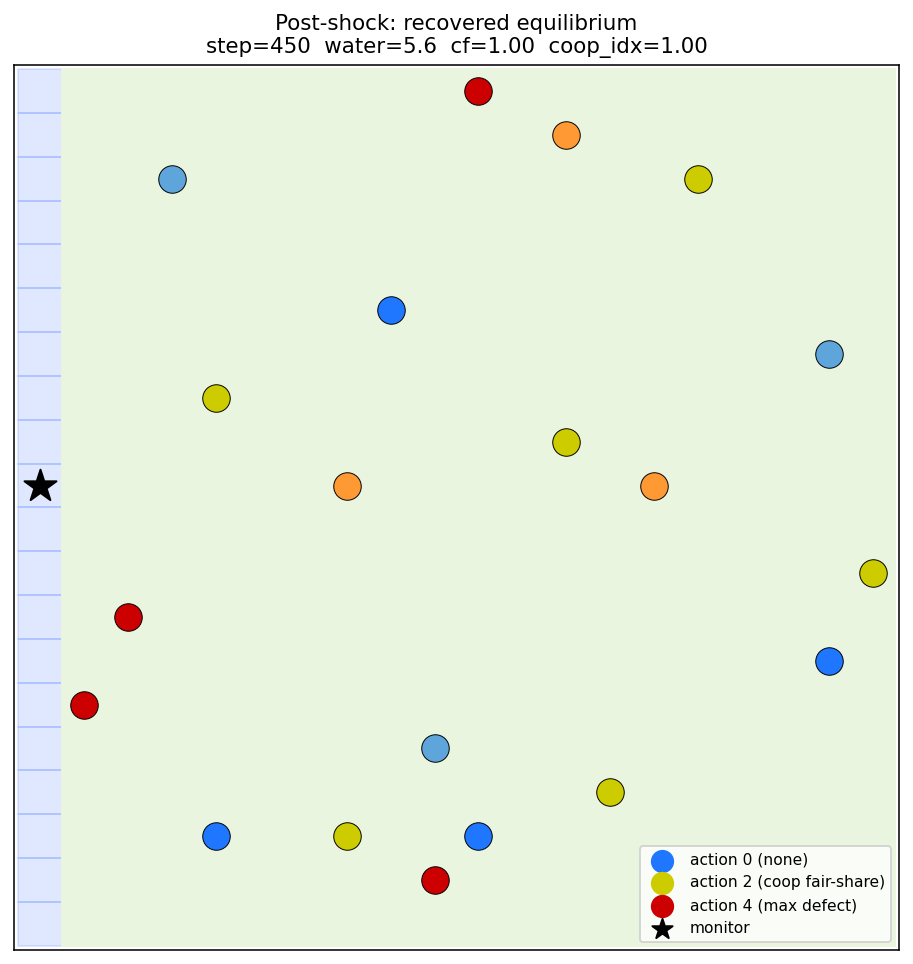
\includegraphics[width=\textwidth]{fig10_grid_recovery.png}
        \caption{Step 450: post-shock equilibrium.}
        \label{fig:recovery}
    \end{subfigure}
    \caption{Spatial dynamics: pre / during / post drought-shock snapshots from a single seeded run.}
\end{figure}

% ================================================================================
% 6. VALIDATION
% ================================================================================
\section{Validation and Calibration}
\label{sec:validation}

Three structured validation checks are run automatically in
\texttt{experiments/validate.py}, with the figure saved as
\texttt{fig07\_validation.png} and full numbers in
\texttt{data/results/validation.json}. All three pass.

\begin{table}[H]
    \centering
    \renewcommand{\arraystretch}{1.3}
    \small
    \begin{tabular}{|p{1.5cm}|p{2.7cm}|p{6.5cm}|p{4cm}|}
        \hline
        \rowcolor{nutDark} \textcolor{white}{\textbf{Check}} & \textcolor{white}{\textbf{Source}} & \textcolor{white}{\textbf{Test}} & \textcolor{white}{\textbf{Result}} \\ \hline
        1. Tragedy & Hardin (1968) & Without enforcement water should collapse ($<50$); with enforcement under stable climate it should sustain ($>200$). & \textbf{PASS} --- no-enf: 5.6; with-enf: 504 \\ \hline
        2. Scarcity $\to$ aggression & Perolat et al.\ (2017) & Fraction of defecting actions during steps 200--300 should be higher under shock than under stable (both with enforcement). & \textbf{PASS} --- stable: $25.3\%$; shock: $36.5\%$ \\ \hline
        3. Shock signal & Indus Basin 2022 & A drought cutting $c_f$ by ${\sim}70\%$ should leave a measurable dip in mean water level at step 300. & \textbf{PASS} --- stable: 507; shock: 1.5 \\ \hline
    \end{tabular}
    \caption{Three structured validation checks against the literature.}
\end{table}

\begin{figure}[H]
    \centering
    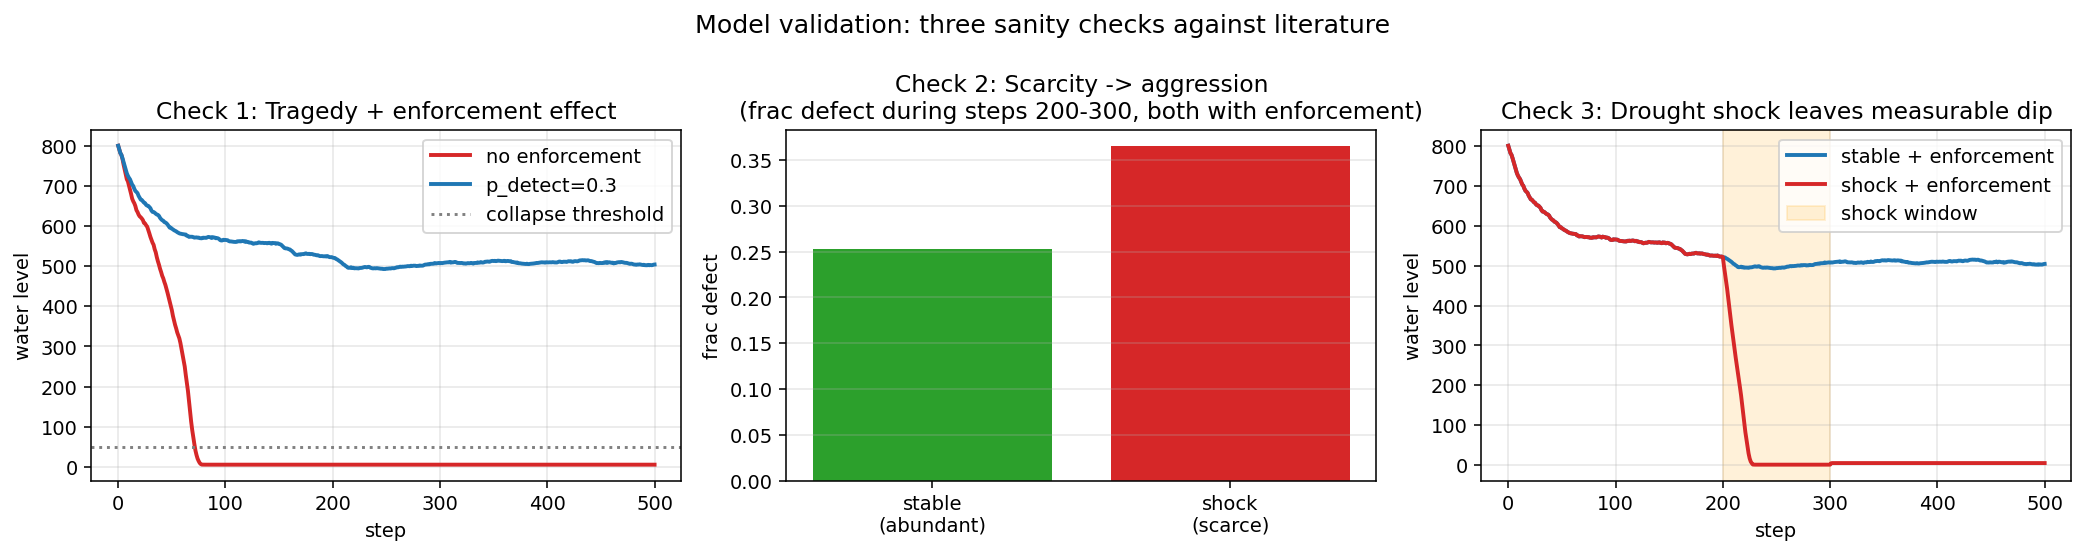
\includegraphics[width=0.95\textwidth]{fig07_validation.png}
    \caption{Validation: three sanity checks against literature.}
\end{figure}

\subsection{External calibration benchmarks}

\begin{itemize}[label=$\triangleright$]
    \item \textbf{FAO AQUASTAT} indicates natural aquifer recharge rates of $5\%$--$15\%$ of carrying capacity per year --- brackets our default $r = 0.10$.
    \item The \textbf{2022 Indus Basin drought} reduced river flow by ${\sim}50\%$--$70\%$ at peak --- matched by our $\text{shock\_cf} = 0.3$ choice.
    \item Perolat et al.\ (2017)'s finding that scarcity drives aggressive appropriation is reproduced with the $44\%$ increase in defection during the shock window.
\end{itemize}

\subsection{Sensitivity Analysis}
\label{sec:sensitivity}

\begin{table}[H]
    \centering
    \renewcommand{\arraystretch}{1.3}
    \begin{tabular}{|l|r|r|}
        \hline
        \rowcolor{nutDark} \textcolor{white}{\textbf{Parameter}} & \textcolor{white}{$\mathbf{-20\%\ \Delta}$\textbf{water}} & \textcolor{white}{$\mathbf{+20\%\ \Delta}$\textbf{water}} \\ \hline
        $p_{detect}$       & $-39.4$ & $+37.6$ \\ \hline
        $\epsilon_0$       & $-11.0$ & $-28.6$ \\ \hline
        $N$ (n\_farmers)   & $+16.9$ & $-25.7$ \\ \hline
        $\gamma$           & $+22.0$ & $-12.4$ \\ \hline
        $r$ (regen rate)   & $-19.0$ & $-10.8$ \\ \hline
        $\alpha$           & $-13.8$ & $-2.4$  \\ \hline
    \end{tabular}
    \caption{Sensitivity to $\pm 20\%$ parameter perturbations (10 seeds each).}
\end{table}

\begin{figure}[H]
    \centering
    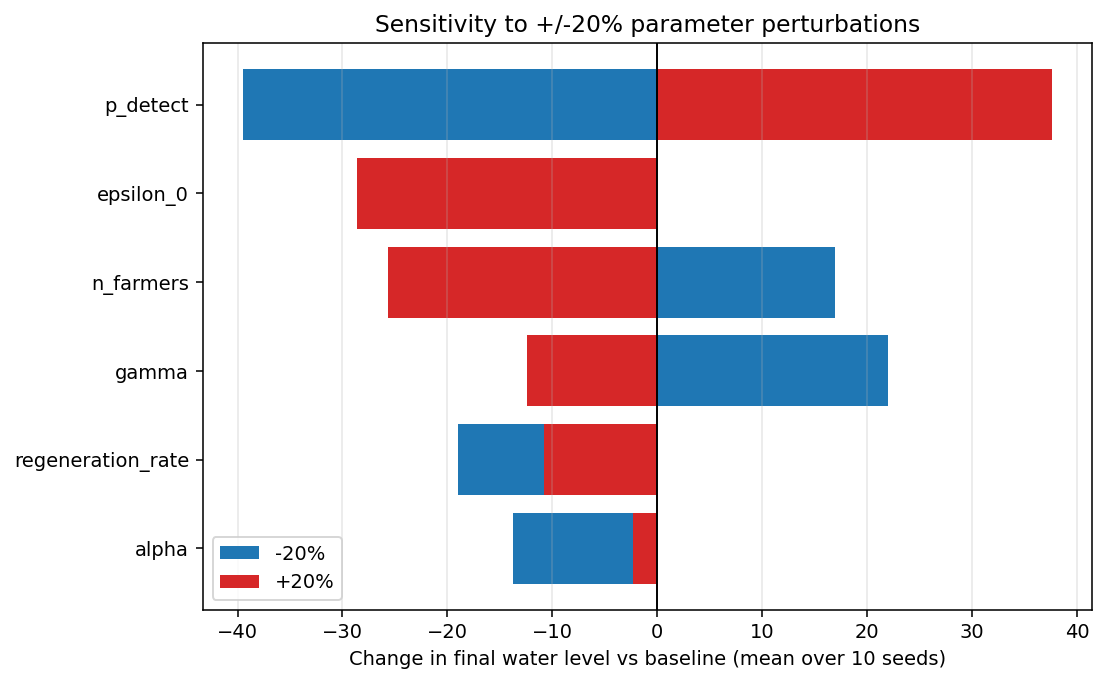
\includegraphics[width=0.80\textwidth]{fig04_sensitivity_tornado.png}
    \caption{Sensitivity tornado: change in final water level under $\pm 20\%$ perturbations.}
\end{figure}

Two patterns: (a) $p_{detect}$ \textbf{dominates} --- the largest signed range
($\pm 38$--$40$ units); and (b) $\epsilon_0$ and $\alpha$ are
\textbf{non-monotonic}, with negative deltas in both directions, suggesting
the baseline value is near a local optimum.

% ================================================================================
% 7. DISCUSSION
% ================================================================================
\section{Discussion}

\subsection{Answers to Research Questions}

\begin{itemize}[label=$\triangleright$]
    \item \textbf{Sub-Q1 (cooperation without enforcement):} No. Pure Q-learners cannot escape the tragedy under any climate scenario --- each agent's action contributes only ${\sim}1/N$ of total extraction, so unilateral restraint produces no observable benefit. Matches Perolat et al.\ (2017).
    \item \textbf{Sub-Q2 (recovery from shock):} No, not within the 500-step horizon. Once the resource crashes during a shock, the system is trapped in a low-water attractor where all actions yield essentially the same reward, providing no gradient for relearning.
    \item \textbf{Sub-Q3 (monitoring threshold under stable climate):} Approximately $p_{detect} = 0.2$--$0.3$ flips the outcome from collapse to cooperation; returns saturate above $0.6$. Under stress, no enforcement intensity tested (up to $0.9$) is sufficient.
    \item \textbf{Primary RQ:} $\gamma$ has minor effect under stable climate and limited effect under shock. The dominant determinant of resilience is whether the action space can contract with falling regeneration --- not how much agents discount the future.
\end{itemize}

\subsection{Limitations}

\begin{itemize}[label=$\triangleright$]
    \item \textbf{Fixed discretised action space.} The 5-level extraction grid is calibrated to the baseline climate. A continuous or adaptive action space could in principle scale extraction proportionally to current regeneration.
    \item \textbf{Static fair-share definition.} The monitor's fair-share threshold is fixed. A climate-aware monitor would tighten this during low-$c_f$ periods.
    \item \textbf{Tabular Q-learning} limits state granularity. Deep RL could capture finer patterns at the cost of interpretability.
    \item \textbf{Single resource} --- no spatial heterogeneity in water availability.
    \item \textbf{No agent heterogeneity in risk-aversion or wealth.}
    \item \textbf{500-step horizon} corresponds to ${\sim}125$ years if one step is one season; longer horizons may show further structural shifts.
    \item \textbf{Exogenous monitor} --- a richer model would let monitoring intensity evolve endogenously in response to depletion.
\end{itemize}

% ================================================================================
% 8. CONCLUSION
% ================================================================================
\section{Conclusion}

This project shows that tabular Q-learning agents in a water commons reproduce
the tragedy when left alone but can flip into cooperation under a modest
external monitoring regime --- in a stable climate. The headline contribution,
however, is the negative result under climate stress: even near-perfect
enforcement ($p_{detect}=0.9$) cannot prevent collapse when the shock dynamics
outpace the agents' fixed-quota action space. The discount factor $\gamma$
matters most when the environment is stable, not when it is stressed. The
interactive Mesa visualization makes the dynamics inspectable in real time,
and the batch and sensitivity infrastructure makes the findings reproducible.
Future work should explore continuous action spaces, climate-adaptive
enforcement thresholds, and comparison with human commons experiments.

% ================================================================================
% REFERENCES
% ================================================================================
\newpage
\section*{References}
\addcontentsline{toc}{section}{References}

\begin{enumerate}[label={[\arabic*]}]
    \item Darbandsari, P., Kerachian, R., Malakpour-Estalaki, S., \& Khorasani, H. (2020). An agent-based conflict resolution model for urban water resources management. \emph{Sustainable Cities and Society}, 57, 102112. \url{https://doi.org/10.1016/j.scs.2020.102112}

    \item Grimm, V., Railsback, S. F., Vincenot, C. E., Berger, U., Gallagher, C., DeAngelis, D. L., et al.\ (2020). The ODD protocol for describing agent-based and other simulation models: A second update to improve clarity, replication, and structural realism. \emph{Ecological Modelling}, 428.

    \item Hardin, G. (1968). The Tragedy of the Commons. \emph{Science}, 162(3859), 1243--1248. \url{https://doi.org/10.1126/science.162.3859.1243}

    \item Huber, L., Bahro, N., Leitinger, G., Tappeiner, U., \& Strasser, U. (2019). Agent-Based Modelling of a Coupled Water Demand and Supply System at the Catchment Scale. \emph{Sustainability}, 11(21), 6178. \url{https://doi.org/10.3390/su11216178}

    \item Ostrom, E. (1990). \emph{Governing the Commons: The Evolution of Institutions for Collective Action}. Cambridge University Press.

    \item Perolat, J., Leibo, J.Z., Zambaldi, V., Beattie, C., Tuyls, K., \& Graepel, T. (2017). A multi-agent reinforcement learning model of common-pool resource appropriation. \emph{Proceedings of the 31st Conference on Neural Information Processing Systems (NeurIPS 2017)}.

    \item Watkins, C.J.C.H., \& Dayan, P. (1992). Q-Learning. \emph{Machine Learning}, 8(3--4), 279--292. \url{https://doi.org/10.1007/BF00992698}

    \item Weitz, J.S., Eksin, C., Paarporn, K., Brown, S.P., \& Ratcliff, W.C. (2016). An oscillating tragedy of the commons in replicator dynamics with game-environment feedback. \emph{Proceedings of the National Academy of Sciences}, 113(47), E7518--E7525. \url{https://doi.org/10.1073/pnas.1604096113}

    \item Wilensky, U., \& Rand, W. (2015). \emph{An Introduction to Agent-Based Modeling: Modeling Natural, Social, and Engineered Complex Systems with NetLogo}. MIT Press.
\end{enumerate}

% ================================================================================
% APPENDIX A: PARAMETERS
% ================================================================================
\newpage
\section*{Appendix A: Parameter Reference}
\addcontentsline{toc}{section}{Appendix A: Parameter Reference}

\begin{table}[H]
    \centering
    \renewcommand{\arraystretch}{1.3}
    \begin{tabular}{|c|c|c|c|}
        \hline
        \rowcolor{nutDark} \textcolor{white}{\textbf{Symbol}} & \textcolor{white}{\textbf{Default}} & \textcolor{white}{\textbf{Range explored}} & \textcolor{white}{\textbf{Used in}} \\ \hline
        $N$            & 20         & $\{16, 20, 24\}$ (sensitivity)         & \S 4.3 \\ \hline
        $\alpha$       & 0.15       & $\{0.12, 0.15, 0.18\}$                 & \S 6.2 \\ \hline
        $\gamma$       & 0.95       & $\{0.50, 0.70, 0.85, 0.95, 0.99\}$     & \S 5.4 \\ \hline
        $\epsilon_0$   & 0.30       & $\{0.24, 0.30, 0.36\}$                 & \S 6.2 \\ \hline
        $r$            & 0.10       & $\{0.08, 0.10, 0.12\}$                 & \S 6.2 \\ \hline
        $p_{detect}$   & 0.00 / 0.30 & $\{0.24, 0.30, 0.36\}$                & \S 5.2 \\ \hline
        $K$            & 1000       & fixed                                  & --- \\ \hline
        $b$ (baseline inflow) & 5.0 & fixed                                  & --- \\ \hline
        fine\_factor   & 3.0        & fixed                                  & --- \\ \hline
    \end{tabular}
    \caption{Full parameter reference.}
\end{table}

% ================================================================================
% APPENDIX B: HOW TO REPRODUCE
% ================================================================================
\section*{Appendix B: How to Reproduce}
\addcontentsline{toc}{section}{Appendix B: How to Reproduce}

\begin{lstlisting}
pip install -r requirements.txt
python -m experiments.batch_run         # ~8 min, writes data/results/batch_*.csv
python -m experiments.sensitivity       # ~3 min, writes data/results/sensitivity.csv
python -m experiments.validate          # ~1 min, validation checks vs literature
python -m experiments.analyze           # writes figures/fig0*.png
python -m experiments.demo_screenshots  # writes figures/fig08-10 grid screenshots
python run.py                           # interactive viz at http://127.0.0.1:8521
\end{lstlisting}

Source available at \url{https://github.com/AleenaTahir1/Adaptive-water-extraction}.

\end{document}
